% $HeadURL: https://sbgn.svn.sourceforge.net/svnroot/sbgn/trunk/documents/specifications/EntityRelationship/Level1/sources/stateVariable.tex $

\color{blue}

\subsection{Glyph: \glyph{State variable}}
\label{sec:stateVariable}

Many biological entities such as molecules can exist in different \emph{states}, meaning different physical or informational configurations.  These states can arise for a variety of reasons.  For example, macromolecules can be subject to post-synthesis modifications, wherein residues of the macromolecules (amino acids, nucleosides, or glucid residues) are modified through covalent linkage to other chemicals.  Other examples of states are alternative conformations as in the closed/open/desensitized conformations of a transmembrane channel, and the active/inactive forms of an enzyme.

SBGN provides a means of associating one or more \glyph{state variables} with an entity; each such variable can be used to represent a dimension along which the state of the overall entity can vary.  When an entity can exist in different states, the state of the whole entity (\ie the SBGN object) can be described by the current values of all its \glyph{state variables}, and the values of the \glyph{state variables} of all its possible components, recursively.

In \SBGNERLone, \glyph{state variables} are also used to describe the localisation in compartments (a transport is therefore described as a state variable assignment, see \sect{assignment}).

\begin{glyphDescription}

\glyphSboTerm Not applicable.

\glyphContainer A \glyph{state variable} is represented by an ''sausage'' container, that is two hemicycles of same radius joined by parallel segments, as shown in \fig{state-var}.  The parallel segment axis should be tangent to the border of the glyph of the \glyph{EN} being modified by the \glyph{state variable}. The center of the bounding box of a \glyph{state variable} should be located on the mid-line of the border of the \glyph{EN}.

\glyphLabel A \glyph{state variable} is identified by a label placed in an unbordered box containing a string of characters.  The characters can be distributed on several lines to improve readability, although this is not mandatory.  The label box must be attached to the center of the container.  The label may spill outside of the container.

\glyphAux A \glyph{state variable} does not carry any auxiliary items.

\end{glyphDescription}

\begin{figure}[H]
  \centering
  \includegraphics[scale = 0.3]{images/stateVariable}
  \caption{The \ER glyph for \glyph{state variable}.}
  \label{fig:state-var}
\end{figure}

A \glyph{state variable} does not necessarily have to be Boolean-valued.  For example, an ion channel can possess several conductance states; a receptor can be inactive, active and desensitized; and so on.  As another example, a \glyph{state variable} ``ubiquitin'' could also carry numerical values corresponding to the number of ubiquitin molecules present in the tail.

The state variable is assigned state-values (see \sect{assignment}). Those values are contained in a glyph similar to the \glyph{stateVariable}, although not carried by another \glyph{EN}.

Two state variables are predefined. The variable \glyph{existence} is used to represent the creation or destruction of entities, as seen on \fig{existence}\label{sec:existence}. \glyph{Existence}   can take two values, true (T) or false (F). The variable is represented by a circle vertically divided in two. One hemicircle is black, and the other white.

\begin{figure}[H]
  \centering
  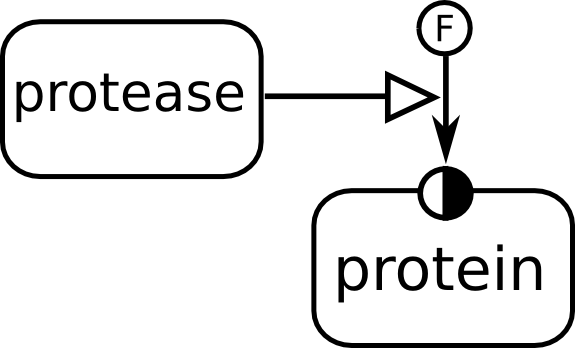
\includegraphics[scale = 0.5]{examples/existence-degradation}
  \caption{Using the \glyph{state variable} \glyph{existence} to represent the degradation of a protein by a protease (i.e. the influence of the protease on the existence of the protein.}
  \label{fig:existence}
\end{figure}

The variable \glyph{location} is used to represent the physical location of an entity, as seen on \fig{location}\label{sec:location}. \glyph{Location} can take any value, but there can be only one \glyph{location} per entity. The variable is represented by a circle containing a slanted pin.

\begin{figure}[H]
  \centering
  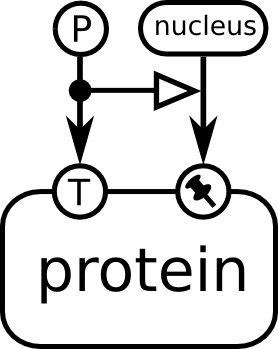
\includegraphics[scale = 0.5]{examples/location-phosphorylation}
  \caption{Using the \glyph{state variable} \glyph{location} to represent the positive effect of a phosphorylation on the nuclear location of a protein (i.e. the influence of a phosphorylation assignment to the nuclear assignment). Note that this does not tell-us anything about the location of protein in the absence of phosphorylation.}
  \label{fig:location}
\end{figure}

\normalcolor

% The following is for [X]Emacs users.  Please leave in place.
% Local Variables:
% TeX-master: "../sbgn_ER-level1"
% End:

